\documentclass[10pt]{article}

% Smaller margins
% \usepackage{fullpage}
\usepackage[margin=0.5in]{geometry}


% cite package, to clean up citations in the main text. Do not remove.
\usepackage{cite}

% Handle images
\usepackage{graphicx}

% Remove brackets from numbering in List of References
\makeatletter
\renewcommand{\@biblabel}[1]{\quad#1.}
\makeatother

\begin{document}

% Remove page number on first page.
\thispagestyle{empty}

% Title
\begin{flushleft}
    {\Large
        \textbf{Iterative strategy for discovering \textit{in vitro} directed cell state transitions using combinatorial activation and repression of endogenous genomic loci}
    }
    \\
    Gleb Kuznetsov | Biophysics 205 Final Project Proposal | April 28, 2015
\end{flushleft}

\begin{abstract}

Improved strategies for cellular reprogramming and directed differentiation offer to advance the potential for stem cell-based therapies and patient/tissue-specific drug screening. Rational analysis followed by low throughput experimentation has enabled derivation of specific cell types that resemble target types morphologically and functionally. However, these reprogrammed cells do not fully recapitulate their target cell types in many cases. On a molecular level, most induced cell lines have been shown to harbor signatures of their originating cells \cite{cahan2014cellnet}, which may ultimately limit their stability and therapeutic potential. I propose leveraging advances in writing cell epigenetic state to combinatorially explore reprogramming and directed differentiation pathways with the goal of identifying cell fate modification programs that are less constrained by assumptions and knowledge \textit{a priori}. I describe an iterative strategy for discovering such pathways. This strategy leverages catalytically dead Cas9 (dCas9) fused to activating or repressing domains (and simultaneous use of orthogonal dCas9's with respective fusions) along with a combinatorial library of guide RNA arrays simultaneously targeting activation and/or repression of multiple genomic loci. Fluorescence-activated cell sorting (FACS) provides a high-throughput means of assaying progress towards a goal and RNA-seq, both targeted and single cell, in combination with computational means of inferring cell state from transcription data, allows for closing the gap between reprogrammed and target cell state.

\end{abstract}

\section*{Introduction}

Better strategies for deriving cell types of interest in vitro will play a central role in regenerative therapies and patient- and tissue-specific drug screening. The field of reprogramming gained much attention with the first successful cloning of a mammal nearly two decades ago \cite{campbell1996sheep}. A decade later, it was shown that it is sufficient to induce somatic cells into an embryonic-like state through the ectopic expression of just four factors: Oct4, Sox2, Klf4, and c-Myc (OSKM) \cite{takahashi2006induction}, now commonly referred to as the Yamanaka factors. Today there exists a multitude of examples of somatic cells being reprogrammed to pluripotent stem cell state and further examples of cell reprogramming to various progenitor and terminate cell fates.

Still, while the reported programmed cell types may resemble their target types on a morphological, functional, and molecular level to some extent, imperfections in both the process of deriving these cells and cell line products remain obstacles in the pursuit of therapies and drug screening efforts. A commonly employed technique for reprogramming, the overexpression of ectopic factors, is limited in throughput and results in the integration of exogenous genetic material into the genome of a cell, increasing the risk of using the resulting cells in human therapies and potentially confounding the results of drug screening studies. Methods that avoid viral integration through the use of mRNAs \cite{warren2010highly}, are technically more complex and lower throughput, limiting their potential as a platform for discovering reprogramming pathways. A pair of complementary studies recently reported that most engineered cell lines examined still carry significant signatures of the cell lines they originated from \cite{cahan2014cellnet, morris2014dissecting}. The software platform at the core of these studies, CellNet, infers the gene regulatory networks (GRNs) active in a cell, which serves as the gold standard for quantitative representation of cell fate \cite{davidson2006gene}. Despite reporting a mismatch in cell state, CellNet also offers a path forward by recommending potential target factors for up- or down-regulation in subsequent engineering efforts.

While this iterative process of overexpressing or knocking down targets recommended by CellNet was demonstrated to be fruitful, for example for improving B cell to macrophage conversion \cite{morris2014dissecting}, recent advances in technologies to perturb cell epigenetic state potentially offer a higher throughput way forward. The CRISPR-Cas9 system is an RNA-programmable homing device for precisely targeting endonuclease activity to genomic loci of interest. The nuclease activity of the Cas9 protein may be inactivated yielding a catalytically dead Cas9 (dCas9) which can then be further fused to activation or repression domains, yielding a tool for precise epigenetic control \cite{qi2013repurposing}. Several recent advances have improved the activating strength of dCas9-activating domain fusions \cite{konermann2014genome, chavez2015VPR}, yielding a tool that enables physiologically relevant levels of activation of endogenous loci. Additionally, the CRISPR-Cas9 system is naturally multiplexable through the specification of multiple guide RNAs (gRNAs). Finally, orthogonal Cas9 proteins have been reported \cite{esvelt2013orthogonal}, enabling simultaneous programming and execution of functions of different nature (e.g. activation and repression). All of this, in combination with advances in methods for combinatorial assembly of DNA constructs, reveals a system for combinatorially exploring perturbations of epigenetic cell state.

The ability to limit the space of combinations to test through a quantitative understanding of cell GRNs enabled by CellNet and the availability of highly programmable dCas9-effector domain fusions presents an opportunity for an iterative, high-throughput method for improving cell reprogramming and directed differentiation. I describe the development and application of this method in a series of four aims of increasing complexity and discovery potential: In \textit{Aim 1}, I focus only on testing combinations of TF activation and validate through an experiment to ``rediscover'' the Yamanaka factors in the induction of mouse embryo fibroblast to pluripotent embryonic stem cell-like fate \cite{takahashi2006induction}. In \textit{Aim 2}, I develop the ability to simultaneously search over activation and repression combinations by leveraging orthogonal dCas9 \cite{esvelt2013orthogonal} fusions with activation and repression effectors and validate in the context of B cell to macrophage conversion. Finally, in \textit{Aim 3}, I describe an open ended method of hierarchically discovering de novo reprogramming pathways through searching a large combinatorial space of activation and repression combinations and assaying for the appearance of cell state markers of increasing terminality in successive rounds of experimentation.

%In \textit{Aim 3}, I apply the system to the as yet unresolved problem of converting fibroblasts to hepatocytes. Finally, in \textit{Aim 3}, I describe a highly speculative method of hierarchically discovering de novo reprogramming pathways through searching a large combinatorial space of activation and repression combinations and assaying for the appearance of cell state markers of increasing specificity in successive rounds of experimentation.

Experiments are carried out in mouse to leverage the datasets already available in CellNet \cite{cahan2014cellnet} and to be able to reproduce previously reported reprogramming and directed differentiation results in developing this method.

\section{Aim 1: Test combinatorial gene activation only and validate by ``rediscovering'' Yamanaka factors.}

The purpose of \textit{Aim 1} is to test only combinatorial gene activation using a dCas9-activator domain fusion and to demonstrate the major steps in the iterative strategy which is the essence of the full method described in this proposal. To validate and tune the method, I will use the exercise of ``rediscovering'' the Yamanaka reprogramming factors Oct4, Sox2, Klf4, and c-Myc (OSKM) that were shown to induce mouse embryonic fibroblasts into a pluripotent state \cite{takahashi2006induction}.

\begin{figure}
\centering
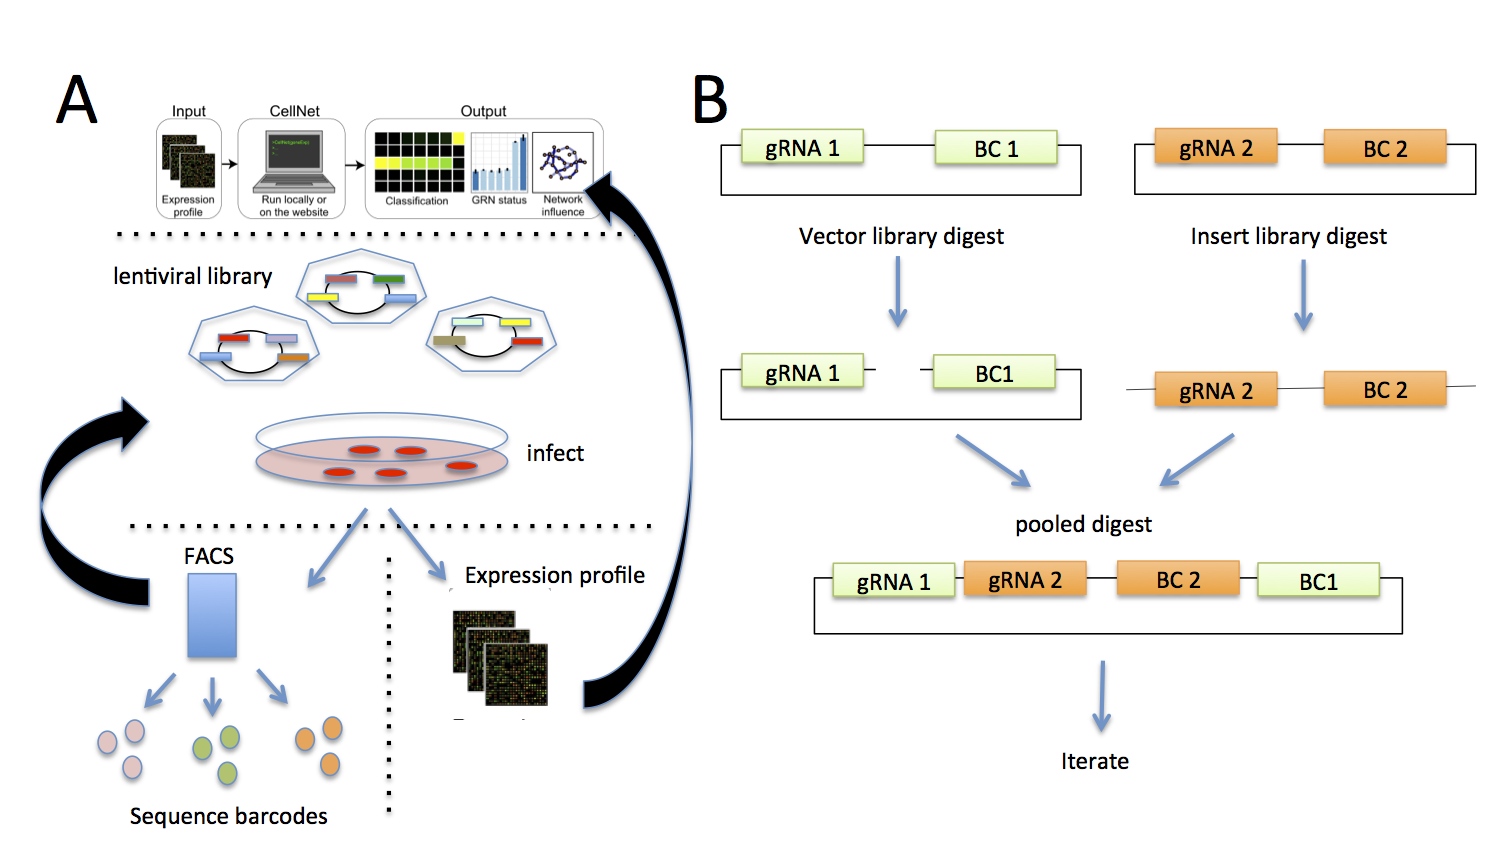
\includegraphics[width=\textwidth]{fig1}
\caption{\textit{(A)} Overview of iterative reprogramming approach using lentiviral library composed of combinatorial gRNAs. \textit{(B)} Combinatorial cloning strategy based on CombiGEM\cite{cheng2014enhanced}.}
\label{fig1}
\end{figure}

Figure \ref{fig1} shows a general overview of the approach consisting of the following steps:
\begin{enumerate}
    \setlength{\itemsep}{0pt}
    \item{Identify the candidate transcription factors for which we'll test combinations. For rediscovering the Yamanaka factors, we will start with the original 24 initial candidates reported in that work \cite{takahashi2006induction}.}
    \item{Prepare lentiviral library containing combinations of the transcription factors.}
    \item{Infect and incubate.}
    \item{Harvest cells and sort using FACS, targeting markers important in target cell type.}
    \item{Sequence barcodes for each well and iterate on lentiviral library. Repeat steps 3-5 several times.}
    \item{RNA-sequencing and CellNet on final products to identify GRN state. Use this information to update lentivirus library.}
\end{enumerate}

\subsection{General Design Decisions}

There are a few design decisions to make \textit{a priori} but these will likely need to be tuned throughout developing the method. One decision is which dCas9-activator fusion to use. Two systems were recently reported: an engineered dCas9-activator system designed by inspecting dCas9 structure from the Zhang Lab \cite{konermann2014genome} and a dCas9 fused to a tripartite activator, VP64-p65-rta (VPr) from the Church Lab \cite{chavez2015VPR}. Both were shown to have as much as four orders of magnitude-fold activation over baseline expression for some targets. Another option, rather than using dCas9-activating domain fusion, is to use an activating dCas9-acetyltransferase fusion which catalyzes acetylation of histone H3 lysine 27 at its target sites, leading to robust transcriptional activation of target genes from promoters and both proximal and distal enhancers \cite{hilton2015epigenome}.

Another design decision to make in advance is how many gRNAs to test in parallel. This decision is constrained by the decreasing activation effect with increasing target multiplexity demonstrated in the dCas9-activator reports mentioned above, by the method for constructing the gRNA-barcode constructs according to the CombiGEM \cite{cheng2014enhanced} strategy (detailed below), as well as the combinatorial library size to explore. Guided by the \textit{Aim 1} context of rediscovering the four Yamanaka factors and the highest multiplicity reported for CombiGEM so far of four elements, I will use cassettes consisting of four guide RNAs.

Finally, another design decision is what multiplicity of infection (MOI) to use for lentivirus infection. For simplicity, I will start with a MOI of one, although increasing this number increases the opportunities for testing combinations of higher numbers, if not exhaustively.

\subsection{Controls}

Given knowledge of the OSKM ``solution'' to the search for the Yamanaka factors, a positive control will involve carrying out the steps of the experiment with the individual gRNA component inputs to the combinatorial library construction limited to those targeting only the four OSKM factors. The negative control will be the complementary library that omits gRNAs targeting any of the OSKM factors. One caveat, discussed below under \textit{Risks}, is that it's not clear that a single guide RNA (sgRNA) targeted to the promoter region of any of OSKM is sufficient for adequate activation. To verify adequate expression, I would conduct quantitative PCR and compare to non-transduced cells to verify activation of the target loci.

\subsection{Steps in Depth}

\subsubsection{Identifying candidate transcription factors for screen}

Since the number of transcription factors in the human genome numbers around 2600 \cite{babu2004structure}, it's intractable to search the space of all possible combinations, even at a multiplicity of two. Instead, it is necessary is to computationally assess expression data for the target tissue type and/or leverage CellNet \cite{cahan2014cellnet} to generate a list of candidate nodes that may play a role in establishing the gene regulatory networks for the tissue type.

However, given that \textit{Aim 1} attempts to validate the method, I will artificially narrow the space of candidate transcription factor targets to the 24 candidates originally targeted by Takahashi and Yamanaka \cite{takahashi2006induction}. One caveat to be aware of is that it may be necessary to include multiple gRNAs for a particular locus, which complicates the combinatorial story a bit.

\subsubsection{Constructing combinatorial lentiviral library}

Genetic constructs will be delivered to cells by lentivirus transduction. The choice of lentivirus for delivery is guided by the opportunity to have reasonable control over multiplicity of infection through modulating virus titer vs cell concentration, as well as stable integration of the payload, enabling propagation throughout cell progeny. The payload delivered by a given lentivirus includes a an array of gRNAs, an array of corresponding barcodes that uniquely identify the combination and order of gRNAs, the dCas9-activator fusion, and a selectable marker for being able to purify out cells that are successfully infected by at least one lentivirus.

To construct the combinatorial library of gRNA and barcodes, I will use the strategy of Combinatorial Genetics En Masse (CombiGEM) \cite{cheng2014enhanced} originally developed for use in \textit{E. coli} and recently communicated to function in mammalian cells \cite{lu2015combigem}. Briefly, CombiGEM uses an iterative cloning strategy starting with a library of DNA elements consisting of a gRNA and corresponding barcode. The DNA element includes restriction sites immediately between the gRNA and barcode and on either side. A library of vectors is generated through restricting between gRNA and barcodes and a library of inserts is created from the same source by cleaving around the gRNA and barcode. The vector and insert libraries are combined and ligated, yielding new DNA elements with an array of gRNAs and the corresponding array of barcodes. This process is repeated for each order of multiplexity desired, and was reported to work robustly to at least a multiplexity of four in \cite{cheng2014enhanced}.

\subsubsection{Infection with lentivirus and incubation}

The lentiviral library is delivered to the cells at a calculated multiplicity of infection (MOI). The simplest strategy would be to use an MOI of one; however, increasing the MOI potentially allows testing greater combinations. After some time (48 hours for Yamanaka context), cells are challenged by compound for which selectable marker delivered by lentivirus protects against. Cells are allowed to incubate for more time (48 hours for Yamanaka context), allowing for propagation of expression changes and ideally appearance of reprogrammed cells.

\subsubsection{Harvesting cells and FACS}

Knowledge of the target GRNs informs selection of antibodies bound to fluorophores for FACS. For the Yamanka factor rediscovery experiment, there are many commercially available kits for assaying induced pluripotent stem cells. These include target markers of pluripotent state such as OCT4, SOX2, SSEA4, and TRA-1-60. The appropriate markers should be determined based on the cell type of interest. It may be possible to use multiple sorting channels to distinguish expression of varying intensity.

\subsubsection{Sequencing barcodes, designing next lentiviral library}

Following FACS, the barcode regions are amplified using pre-designed PCR primer adapters \cite{cheng2014enhanced} and the barcodes are read using next generation sequencing. The resulting data is then analyzed for enrichment of targeted factors. Based on enrichment, the lentiviral library is redesigned to over-represent the enriched factors. Repeat steps 3 - 5 several times until no significant change in enrichment is observed.

\subsubsection{Transcriptional profiling, inferring GRNs}

After the final iteration of lentiviral infection, the best expressing cells as assessed by FACS can be transcriptionally profiled. The choice of technology depends on availability. Bulk chip or RNA-seq may be adequate given the sorting carried out, but single cell RNA-seq may yield insights that bulk sequencing does not, especially directly connecting expression to specific barcode. Comparing the GRN of these final cells to the target GRN state may inform additional factors to test, which may have been left out of the original screen. A new lentiviral library can then be redesigned and infection and sorting and/or transcriptional profiling repeated.

\subsection{Risks}

\textbf{Activation efficiency}: dCas9-activating domain fusions have only been characterized for a handful of factors and already this has shown that the amount of activation depends on the gene as well as the specific gRNA target \cite{chavez2015VPR, konermann2014genome}. Additionally, activation fold falls with increasing multiplexity. Nonetheless, it has been shown that a single guide RNA is sufficient for significant activation of several factors \cite{konermann2014genome}.
\newline

\noindent \textbf{Calibrating lentivirus multiplicity of infection}: The current bulk barcode sequencing strategy does not give a way to test multiplicity of infection.
\newline

\noindent \textbf{Biological limitations}: It might be possible that certain loci are inaccessible due to chromatin state and none of the starting pool of transcription factors can serve as an adequate pioneer factor to initiate transition.

\section{Aim 2: Implement searching over combinations of activation and repression}

In this aim, I add multimodality to the combinatorial method developed in this proposal, introducing the ability to simultaneously activate and repress different loci. To validate this method, I use  B cell to macrophage conversion, a relatively quick (10 hours) and robust conversion that has been reported to only require a single transcription factor C/EBP$\alpha$ \cite{bussmann2009robust}. However, CellNet analysis revealed that a higher fidelity conversion analysis additionally required the knockdown of Pou2af1 and Ebf1 \cite{morris2014dissecting}. The requirement of simultaneous up- and down-regulation, small number of factors, and rapid conversion reduces the variables in testing a multimodal combinatorial strategy.

To allow simultaneous activation and repression of different loci, I will create orthogonal dCas9s based on orthogonal Cas9 proteins reported in \cite{esvelt2013orthogonal}. Orthogonal Cas9 proteins, which recognize different RNA scaffolding structures and different PAM sequences, allow simultaneously carrying out different functions on distinct targets in the genome. The corresponding gRNA library designs must be designed to use the correct scaffolding RNA elements (crRNA and tracrRNAs) for their respective dCas9.

CellNet will be used to specify which factors in the original cell type should be down-regulated and which should be up-regulated. For validating \textit{Aim 2}, this should include the solution factors found, but also include additional factors in order to show that a solution can be found. Two separate lentiviral libraries will be created, one for activation and the other for repression. Infection can be carried out in parallel. Despite looking for combinations of both activation and repression, it's not necessary that all cells get both as even just infection with an activating library may bring a cell type closer to the target.

A caveat that arises here is that the current strategy doesn't allow for identifying which pairs of up-regulation and down-regulation libraries co-occur. Still, limiting the library based on iteration as in \textit{Aim 1} should help clarify this.

\subsection{Controls}

Similar to the Yamanaka system above, as a negative control I would leave out the solution elements C/EBP$\alpha$ as activator targets and Pou2af1 and Ebf1 as repressor targets and look for underrepresentation of macrophage factors in FACS. As a positive control, I would construct libraries enriched the previously left-out factors and expect higher proportion of converted cells.

\subsection{Risks}

\noindent \textbf{How orthogonal is orthogonal?}: Are the Cas9s truly orthogonal with respect to binding their target gRNAs?
\newline

\noindent \textbf{Multiple infection by lentivirus}: Are there issues that arise from multiple lentivirus infection?


% \section{Aim 3: Apply method to differentiation of mouse fibroblasts to hepatocytes}

% In this aim, I apply the method full combinatorial method describe above to attempt to derive better hepatocytes than have previously been developed \cite{huang2011induction, sekiya2011direct}. CellNet was used to show that induced hepatocytes (iHeps) derived in \cite{sekiya2011direct} were actually induced endoderm progenitors, capable of further differentiation toward both liver and intestine \cite{morris2014dissecting}. Unlike Sekiya

% In this aim, I will start with de novo recommendations from CellNet for factors that should be respectively up- or down-regulated.

% The final comparison will be to perform transcriptional profiling (ideally single cell RNA-Seq) and compare inferred GRNs to that of actual liver tissue.

\section{Aim 3: Hierarchical discovery of do novo reprogramming pathways}

This aim is intentionally open-ended and involves pushing the limits of the iterative method developed in this proposal. The goal is to identify novel pathways for directed differentiation by assaying for increasingly differentiated cell types in subsequent rounds of lentiviral library design, infection, and FACS.

The process start with a set with mouse embryonic stem cells and a large library of gRNAs. The same locus may be targeted for activation and repression in the orthogonal lentiviral libraries. Activating gRNAs should be enriched for pioneer factors, as well as factors that serve as hubs in more GRNs. The cycles of lentiviral library design, infection, and FACS is carried out as before, with the additional detail of udpating the set of antibodies using FACS to select for increasingly differentiated cell types. In the first run of FACS, a broad set of antibodies are chosen, specific to general lineage specification marks, e.g. unique markers for endoderm, ectoderm and mesoderm. Following FACS, the respective barcodes in each bucket should be enriched for their respective fate specification. Three new pools of lentiviral factors are created, each respectively enriched for markers in the respective endoderm, ectoderm, and mesoderm buckets. The process is then repeated for the three separate pools. For each pool, a different set of the next-most differentiated antibody types is selected. The branching factor of this process starts to get large so only the most interesting lineages can be followed, to be chosen based on the most promising hits in subsequent rounds.

\subsection{Controls}

As a positive control, use limited libraries targetting endoderm, ectoderm, and mesoderm lineage-specific factors to ensure enrichment of these types. As a negative control, target only a single lineage factor, to ensure that other lineages are not spurious hits.

\subsection{Risks}

\noindent \textbf{Large library size}: The size of the initial gRNA (TBD) may be too large to find a tractable solution. Still, individual factors may be enough to push down interesting paths.

\section*{General Caveats}

\subsection*{Role of Cell Environment}

The environment of cells is known to play an important role in cell fate \cite{drummond2008stem}. The experiment setup in this proposal does not take this into account at the moment. It may be possible that obtaining a particular cell type requires the surrounding environment, including cells and physical setup, to be of a certain distribution of cells.

\subsection*{Relative expression}

As designed, the strategy in the current proposal has not taken into account how to tune relative expression of factors. The effect of dCas9-effector fusions depends on gene context and choice of gRNA, among other factors \cite{konermann2014genome, chavez2015VPR}. The relative expression of each factor, especially during transition, likely matters and may not be evidenced by the final relative expression observed in the target cell type.

\subsection*{Role of temporal expression}

The strategy in this proposal does not take into account the temporal dimension of transcription factor expression. One step in the right direction is to recapitulate development by using multiple lentiviral libraries that contain orthogonal dCas9-effector fusions that are also orthogonally inducible, allowing sequential expression.


% \section*{Future opportunities}

% \textbf{Leverage single-cell targeted RNA-seq}

% The method described in this proposal would benefit from increasing resolution of transcription. Depending on limitations of technology, it may not be necessary to do full genome RNA-seq, but instead to do targeted capture on loci of interest, in consideration of cost. Technologies like Cell-Seq and others could be of use here. If this method is made accessible, it may be interesting to generate many perturbed cells, and just explore the landscape of regulation. Something about forward genetics or forward genomics.

\pagebreak

\bibliographystyle{unsrt}
\bibliography{final_proposal}

\section*{Statement of Outside Help}

\noindent Daniel Goodman (PhD student, Church Lab) - Conversation regarding synthesizing combinatorial gRNA cassette libraries. Discussed limitations on Chip-based synthesis, as well as strategies (barcodes, etc.) for read-out.
\newline

\noindent Alex Ng (PhD student, Church Lab) - Conversation regarding issues related to combinatorial targeting using dCas9-activating domain fusion. Alex pointed out that activation strength for any given promoter is some amount relative to the baseline of that promoter.
\newline

\noindent Pierce Ogden (PhD student) - Conversation regarding lentiviral libraries.

\end{document}
